\documentclass[preprint,3p,number]{elsarticle}

\usepackage{amsmath}
\usepackage{amssymb}
\usepackage{subcaption}
% \usepackage{hyperref}
\usepackage{graphicx}
\usepackage{tikz}
\usepackage{pgfplots}
\usepackage{booktabs}
\usepackage{siunitx}
\usepackage[noabbrev,capitalize]{cleveref}
\usepackage{lipsum}

% Tikz libraries
\usetikzlibrary{arrows.meta,patterns,calc}

\bibliographystyle{elsarticle-num}

\begin{document}

\title{Natural convection flow of an air-filled cavity containing two circular heated cylinders}
\maketitle

\section{Objective}

\begin{itemize}
    \item Establish a verified baseline for natural convection around two
    internal heated cylinders.
\end{itemize}

\section{Goal}

\begin{itemize}
    \item Mesh-converged mean Nusselt numbers for both cylinders
    (changes below $1\%$), a global heat imbalance below $0.1\%$, and documented
    flow and temperature fields over the selected Rayleigh-number range.
\end{itemize}

\section{Problem configuration}

\begin{figure}[htbp]
    \centering
    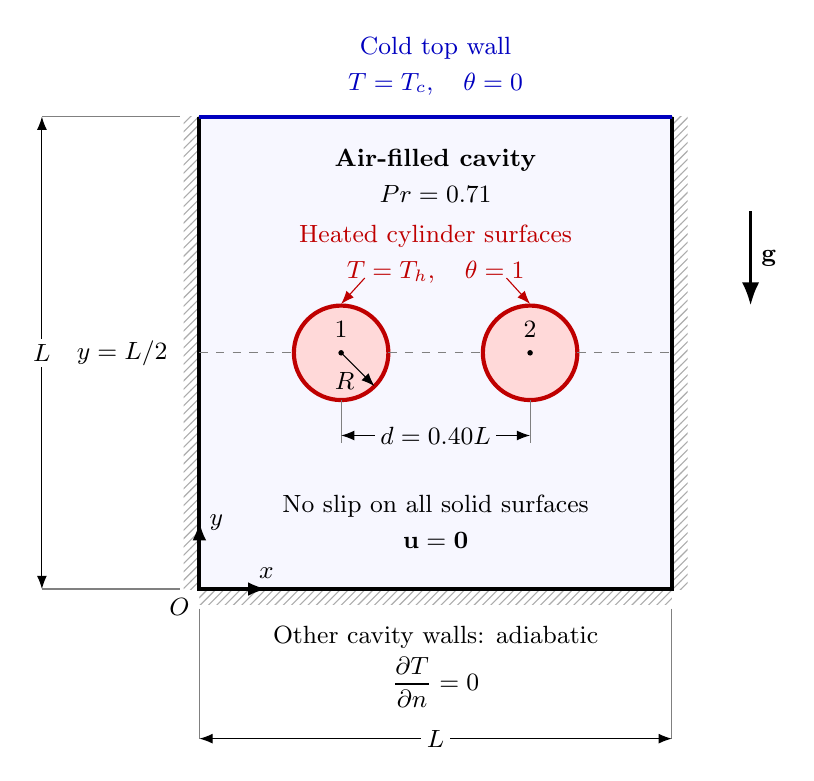
\begin{tikzpicture}[
        >=Latex,
        font=\small,
        wall/.style={line width=1.5pt},
        dimension/.style={<->,thin},
        extension/.style={thin,gray}
    ]
        % Drawing dimensions: L = 6, R/L = 0.10
        \def\L{6}
        \def\R{0.6}
        \coordinate (C1) at (1.8,3);
        \coordinate (C2) at (4.2,3);

        % Air-filled cavity
        \fill[blue!3] (0,0) rectangle (\L,\L);

        % Insulation: left, right, and bottom walls
        \fill[pattern=north east lines,pattern color=gray!65]
            (-0.20,0) rectangle (0,\L);
        \fill[pattern=north east lines,pattern color=gray!65]
            (\L,0) rectangle (6.2,\L);
        \fill[pattern=north east lines,pattern color=gray!65]
            (0,-0.20) rectangle (\L,0);

        % Outer walls
        \draw[wall] (0,\L) -- (0,0) -- (\L,0) -- (\L,\L);
        \draw[wall,blue!75!black] (0,\L) -- (\L,\L);

        % Heated cylinders
        \filldraw[fill=red!15,draw=red!75!black,wall]
            (C1) circle (\R);
        \filldraw[fill=red!15,draw=red!75!black,wall]
            (C2) circle (\R);

        \fill (C1) circle (1pt);
        \fill (C2) circle (1pt);

        \node[above=2pt] at (C1) {$1$};
        \node[above=2pt] at (C2) {$2$};

        % Radius
        \draw[->] (C1) -- ++(-45:\R)
            node[midway,below left,inner sep=1pt] {$R$};

        % Midheight guide
        \draw[dashed,gray] (0,3) -- (1.2,3);
        \draw[dashed,gray] (2.4,3) -- (3.6,3);
        \draw[dashed,gray] (4.8,3) -- (6,3);
        \node[left=8pt] at (0,3) {$y=L/2$};

        % Centre-to-centre spacing
        \draw[extension] (1.8,2.4) -- (1.8,1.85);
        \draw[extension] (4.2,2.4) -- (4.2,1.85);
        \draw[dimension] (1.8,1.95) -- (4.2,1.95)
            node[midway,fill=blue!3,inner sep=2pt]
            {$d=0.40L$};

        % Thermal boundary labels
        \node[above,align=center,text=blue!75!black]
            at (3,6.15)
            {Cold top wall\\[2pt]$T=T_c,\quad \theta=0$};

        \node[align=center,text=red!75!black] at (3,4.25)
            {Heated cylinder surfaces\\[2pt]
             $T=T_h,\quad \theta=1$};

        \draw[->,red!75!black] (2.1,3.95) -- (1.8,3.62);
        \draw[->,red!75!black] (3.9,3.95) -- (4.2,3.62);

        \node[below,align=center] at (3,-0.35)
            {Other cavity walls: adiabatic\\[2pt]
             $\displaystyle \frac{\partial T}{\partial n}=0$};

        % Fluid and no-slip conditions
        \node[align=center] at (3,5.25)
            {\textbf{Air-filled cavity}\\[2pt]$Pr=0.71$};

        \node[align=center] at (3,0.85)
            {No slip on all solid surfaces\\[2pt]
             $\mathbf{u}=\mathbf{0}$};

        % Gravity
        \draw[->,very thick] (7,4.8) -- (7,3.6)
            node[midway,right] {$\mathbf{g}$};

        % Coordinate axes
        \draw[->,thick] (0,0) -- (0.85,0)
            node[above] {$x$};
        \draw[->,thick] (0,0) -- (0,0.85)
            node[right] {$y$};
        \node[below left] at (0,0) {$O$};

        % Cavity dimensions
        \draw[extension] (0,-0.25) -- (0,-1.9);
        \draw[extension] (6,-0.25) -- (6,-1.9);
        \draw[dimension] (0,-1.9) -- (6,-1.9)
            node[midway,fill=white,inner sep=2pt] {$L$};

        \draw[extension] (-0.25,0) -- (-2,0);
        \draw[extension] (-0.25,6) -- (-2,6);
        \draw[dimension] (-2,0) -- (-2,6)
            node[midway,fill=white,inner sep=2pt] {$L$};
    \end{tikzpicture}

    \caption{Step1A: natural convection in an air-filled square
    cavity containing two identical heated circular cylinders.
    The cylinder radius is $R=0.10L$, and their centres are
    $(0.30L,0.50L)$ and $(0.70L,0.50L)$.
    The top wall is cold, while the remaining cavity walls
    are adiabatic. All solid surfaces are stationary and
    impermeable.}
    \label{fig:step1A_setup}
\end{figure}

\end{document}